% !TEX program = xelatex
% ============================================================
%  Gemma-4 E2B 零样本目标检测评测与跨范式对比分析
%  编译方式: xelatex report.tex (编译两遍以更新目录和引用)
% ============================================================
\documentclass[12pt, a4paper]{article}

% ---- 中文支持 ----
\usepackage[UTF8, fontset=windows]{ctex}

% ---- 基础宏包 ----
\usepackage[margin=2.5cm, headheight=14pt]{geometry}
\usepackage{amsmath, amssymb}
\usepackage{graphicx}
\usepackage{booktabs}
\usepackage{hyperref}
\usepackage{enumitem}
\usepackage{xcolor}
\usepackage{float}
\usepackage{caption}
\usepackage{subcaption}
\usepackage{multirow}
\usepackage{array}
\usepackage{fancyhdr}
\usepackage{setspace}

% ---- 页面设置 ----
\pagestyle{fancy}
\fancyhf{}
\fancyhead[L]{\small Gemma-4 零样本目标检测评测}
\fancyhead[R]{\small \thepage}
\renewcommand{\headrulewidth}{0.4pt}

\setstretch{1.3}

% ---- 超链接样式 ----
\hypersetup{
    colorlinks=true,
    linkcolor=blue!70!black,
    urlcolor=cyan!70!black,
    citecolor=green!50!black,
}

% ---- 列表样式 ----
\setlist{nosep, leftmargin=2em}

% ---- 自定义命令 ----
\newcommand{\PLN}{\textsc{PLN}}
\newcommand{\mAPval}{\text{mAP}}
\newcommand{\eg}{\textit{e.g.}}

% ============================================================
\title{%
  \vspace{-1.5cm}
  \textbf{Gemma-4 E2B 零样本目标检测评测与跨范式对比分析} \\[6pt]
  \large Zero-Shot Object Detection with Gemma-4 on Pascal VOC 2007
}
\author{\textbf{种子2301 席佳伟}}
\date{\today}

\begin{document}

\maketitle
\thispagestyle{fancy}

% ============================================================
\begin{abstract}
视觉语言模型VLM的快速发展正在改变目标检测的范式。传统检测器依赖大量标注数据进行有监督训练，而 VLM 通过预训练阶段积累的视觉-语言对齐能力，有望实现零标注成本的目标检测。本报告评测 Google Gemma 4 系列最小模型在 Pascal VOC 2007 上的零样本检测性能。

我使用 有效参数为2.3B 的Gemma-4 E2B-it对 VOC 2007 test 全部 4952 张图进行零样本推理，不做任何微调。设计了包含 prompt 工程、三级容错 JSON 解析、坐标转换、类别模糊匹配和 token log-prob 置信度评估在内的完整评测管线。使用与 PLN 复现项目完全一致的 \texttt{voc\_eval.py} 计算 mAP@0.5，确保跨范式对比的公平性。

Gemma-4 E2B 取得 \textbf{51.51\%} mAP@0.5（mAP@0.75 = 30.05\%），推理成功率 99.5\%。与使用完整有监督训练的 PLN-ResNet18（68.74\%）相差 17.23 个百分点。逐类对比揭示 VLM 在语义特征鲜明的大物体上（cat 90.89\%）可超越专用检测器，但在小目标和密集实例上存在系统性短板。错误分析表明，29.7\% 的 GT 漏检和 16.8\% 的背景误检（幻觉）是主要的性能瓶颈，而非定位精度本身。两种范式在能力维度上呈现互补特征：有监督检测器擅长精确空间定位，VLM 擅长语义理解和零样本泛化。
\end{abstract}

\tableofcontents
\newpage

% ============================================================
\section{引言}

\subsection{任务背景}

在上一个任务中，我复现了 Point Linking Network，将 Backbone 从 Inception-v2 替换为 ResNet-18，在 VOC 2007 Test 上取得 68.74\% mAP@0.5。第二阶段的任务是：使用 Gemma 4 最小模型，在同一数据集上评测零样本 mAP。

两个阶段使用同一数据集、同一评测指标、同一份 \texttt{voc\_eval.py} 评测代码，目的是希望\textbf{在同一把尺子下量化"有监督专用检测"与"零样本通用检测"的差距}，建立对目标检测范式演进的直观认知。

\subsection{零样本检测的意义}

传统目标检测的工作流程是：收集数据 $\to$ 标注边界框 $\to$ 训练模型 $\to$ 部署推理。其中数据标注是最大的成本瓶颈——VOC 2007+2012 的 16k 张标注图在今天看来规模很小，但 COCO 的 120k 张标注成本已经相当可观，而自动驾驶场景的标注成本更是量级级的增长。

VLM 的零样本检测提供了一种完全不同的路径：模型在大规模图文数据上预训练后，无需任何任务特定标注，仅通过自然语言 prompt 即可执行检测。这种能力的实用价值在于：

\begin{itemize}
    \item \textbf{零标注成本}：新类别、新场景无需重新标注和训练
    \item \textbf{开放词汇}：不受预定义类别集的限制
    \item \textbf{快速原型验证}：无需训练流程即可评估检测可行性
\end{itemize}

代价同样明确：精度不如专用检测器，推理速度慢两个数量级。我核心目标就是量化这些 trade-off。


% ============================================================
\section{方法设计}

\subsection{Prompt 设计}

\begin{verbatim}
Detect all objects in this image that belong to these categories:
aeroplane, bicycle, bird, boat, bottle, bus, car, cat, chair, cow,
diningtable, dog, horse, motorbike, person, pottedplant, sheep, sofa,
train, tvmonitor.
For each detected object, output a JSON list where each element has
"box_2d" (as [y_min, x_min, y_max, x_max] in range 0-1000) and "label"
(the category name). Only output the JSON list, nothing else.
\end{verbatim}

设计要点：

\begin{enumerate}
    \item \textbf{显式列出全部 20 类}：避免模型遗漏类别或输出非 VOC 类别名称。
    \item \textbf{指定 \texttt{box\_2d} 格式}：这是 Gemma 4 原生训练的检测输出格式（1000$\times$1000 归一化坐标空间），使用模型训练时的原生格式可以最大化检测质量。
    \item \textbf{要求纯 JSON 输出}：减少解析复杂度。实际测试中模型仍会包裹 markdown code fence（\texttt{```json ... ```}），需在解析前去除。
\end{enumerate}

\subsection{输出解析}

模型的自回归文本输出需要经过多级处理才能转化为标准检测框。

\subsubsection{Markdown fence 去除}

Gemma 4 常将 JSON 包裹在 \texttt{```json ... ```} 中。使用正则表达式在 JSON 解析前去除：

\begin{verbatim}
text = re.sub(r"^```(?:json)?\s*\n?", "", text.strip())
text = re.sub(r"\n?```\s*$", "", text.strip())
\end{verbatim}

\subsubsection{三级容错 JSON 解析}

\begin{table}[H]
\centering
\caption{三级容错解析策略}
\label{tab:parsing}
\begin{tabular}{@{}clc@{}}
\toprule
\textbf{级别} & \textbf{策略} & \textbf{实际命中率} \\
\midrule
L1 & 直接 \texttt{json.loads()} 解析整段输出 & $>$99\% \\
L2 & 正则提取 JSON 数组 \texttt{[\{...\}, ...]} & $<$1\% \\
L3 & 逐个提取 JSON 对象 \texttt{\{...\}} & 极少触发 \\
\bottomrule
\end{tabular}
\end{table}

L1 的高命中率说明 Gemma 4 E2B 的指令遵循能力已经相当稳定。三级设计是防御性编程，确保即使模型输出格式异常也能最大限度地提取有效信息。

\subsubsection{坐标转换}

Gemma 4 输出 \texttt{box\_2d} = $[y_{\min}, x_{\min}, y_{\max}, x_{\max}]$，坐标空间为 0--1000 归一化整数，需转换为 VOC 标准的 $[x_{\min}, y_{\min}, x_{\max}, y_{\max}]$ 像素坐标：

\begin{equation}
    x_{\text{pixel}} = \frac{x_{1000}}{1000} \times W, \quad
    y_{\text{pixel}} = \frac{y_{1000}}{1000} \times H
\end{equation}

转换后对框进行合法性校验（正面积），丢弃退化框。

\subsubsection{类别模糊匹配}

VLM 输出的类别名可能与 VOC 标准名不一致。通过三级匹配解决：

\begin{enumerate}
    \item \textbf{精确匹配}：\texttt{dog} $\to$ \texttt{dog}
    \item \textbf{别名表查找}：维护 30+ 条映射，如 \texttt{airplane} $\to$ \texttt{aeroplane}，\texttt{motorcycle} $\to$ \texttt{motorbike}，\texttt{tv} $\to$ \texttt{tvmonitor}
    \item \textbf{子串匹配兜底}：如 \texttt{dining table} $\to$ \texttt{diningtable}
\end{enumerate}

\subsection{置信度评估}

传统检测器直接输出每个框的 confidence score。VLM 的自回归生成没有这一概念，本项目使用 \textbf{token log-probability 的几何平均值}作为序列级置信度：

\begin{equation}
    \text{confidence} = \exp\left(\frac{1}{T} \sum_{t=1}^{T} \log p(x_t \mid x_{<t})\right)
\end{equation}

其中 $T$ 为生成的 token 数量。该分数反映模型对整段输出的"确定性"，用于 VOC mAP 计算中 precision-recall 曲线的排序。

需要注意的是，这是一个\textbf{序列级}而非\textbf{框级}的置信度——同一张图上的所有检测框共享同一个 score。这是 VLM 做检测的固有限制：框是序列生成的一部分，无法为每个框独立打分。

\subsection{评测协议}

\begin{table}[H]
\centering
\caption{评测配置}
\label{tab:eval_config}
\begin{tabular}{@{}ll@{}}
\toprule
\textbf{项目} & \textbf{配置} \\
\midrule
数据集 & Pascal VOC 2007 test（4952 张，12032 个非 difficult GT 框） \\
指标 & mAP@IoU=0.5（11-point interpolation） \\
评测代码 & \texttt{voc\_eval.py}（与 PLN 项目完全一致） \\
GPU & NVIDIA RTX 4090 (24GB VRAM) \\
精度 & BF16 \\
解码策略 & Greedy（\texttt{do\_sample=False}） \\
最大生成长度 & 2048 tokens \\
断点续传 & 每 50 张保存 checkpoint \\
\bottomrule
\end{tabular}
\end{table}

% ============================================================
\section{实验结果}

\subsection{总体指标}

\begin{table}[H]
\centering
\caption{Gemma-4 E2B 零样本检测总体结果}
\label{tab:overall}
\begin{tabular}{@{}lr@{}}
\toprule
\textbf{指标} & \textbf{数值} \\
\midrule
\textbf{mAP@0.5} & \textbf{51.51\%} \\
总检测框 & 13,191 \\
总 GT 框 & 12,032 \\
平均检测数/张 & 2.7 \\
推理成功率 & 99.50\% (4927/4952) \\
解析失败 & 1 张 (0.02\%) \\
无检测输出 & 24 张 (0.48\%) \\
平均推理时间 & 4.37 s/张 \\
总推理时间 & 360.9 min \\
\bottomrule
\end{tabular}
\end{table}

\subsection{各类 AP 结果}

\begin{table}[H]
\centering
\caption{VOC 2007 Test 全 20 类 AP（Gemma-4 E2B, Zero-shot）}
\label{tab:per_class_ap}
\begin{tabular}{@{}lclclc@{}}
\toprule
\textbf{类别} & \textbf{AP (\%)} & \textbf{类别} & \textbf{AP (\%)} & \textbf{类别} & \textbf{AP (\%)} \\ \midrule
cat & \textbf{90.89} & dog & 82.70 & train & 70.55 \\
horse & 66.61 & cow & 65.11 & bird & 63.71 \\
bus & 61.72 & bicycle & 61.19 & motorbike & 59.86 \\
sheep & 57.84 & person & 53.30 & car & 51.87 \\
aeroplane & 50.55 & tvmonitor & 39.79 & sofa & 36.24 \\
chair & 27.53 & diningtable & 25.08 & boat & 24.86 \\
bottle & 24.00 & pottedplant & \underline{16.86} & & \\
\midrule
\multicolumn{4}{@{}l}{\textbf{mAP = 51.51\%}} \\
\bottomrule
\end{tabular}
\end{table}

\subsection{类别分析}

\textbf{第一梯队（AP $>$ 60\%）}：cat (90.89\%), dog (82.70\%), train (70.55\%), horse (66.61\%), cow (65.11\%), bird (63.71\%), bus (61.72\%), bicycle (61.19\%)。共性特征是物体通常较大、形态特征鲜明、在互联网图像中出现频率高。cat 的 90.89\% 说明 VLM 对这类高辨识度目标的检测能力已经非常强。

\textbf{第二梯队（AP 40--60\%）}：motorbike (59.86\%), sheep (57.84\%), person (53.30\%), car (51.87\%), aeroplane (50.55\%)。person 虽然是最高频类别（约占 GT 的 1/4），但 AP 仅 53.30\%，主要原因是密集场景下 VLM 难以逐个输出所有实例。

\textbf{第三梯队（AP $<$ 40\%）}：tvmonitor (39.79\%), sofa (36.24\%), chair (27.53\%), diningtable (25.08\%), boat (24.86\%), bottle (24.00\%), pottedplant (16.86\%)。弱势类别的共性包括：小目标（bottle, pottedplant），边界模糊的家居物品（chair, diningtable, sofa），以及密集远景目标（boat）。

\subsection{IoU 阈值敏感性分析}

传统检测器的评测通常只报告 mAP@0.5，但这一阈值对定位精度的要求较低。为全面评估 VLM 的空间定位能力，本节在多个 IoU 阈值下重新计算 mAP。

\begin{table}[H]
\centering
\caption{不同 IoU 阈值下的 mAP}
\label{tab:iou_sensitivity}
\begin{tabular}{@{}ccccccc@{}}
\toprule
\textbf{IoU 阈值} & 0.50 & 0.60 & 0.70 & 0.75 & 0.80 & 0.90 \\
\midrule
\textbf{mAP (\%)} & 51.51 & 44.78 & 35.30 & 30.05 & 23.98 & 11.60 \\
\bottomrule
\end{tabular}
\end{table}

从 mAP@0.5 到 mAP@0.75，性能下降了 \textbf{21.46 个百分点}（51.51\% $\to$ 30.05\%），降幅达 41.7\%。作为对比，成熟的有监督检测器（如 Faster R-CNN）从 mAP@0.5 到 mAP@0.75 的降幅通常在 15--25\% 左右。这证实了 VLM 检测的核心短板在于\textbf{空间定位精度}而非语义识别能力。

逐类来看，cat 从 90.89\%@0.5 降至 79.55\%@0.75（降幅 12.5\%），仍然保持在高水平；而 boat 从 24.86\% 暴跌至 6.68\%（降幅 73.1\%），pottedplant 从 16.86\% 降至 5.02\%（降幅 70.2\%）。大物体的定位精度显著优于小物体，这符合 2.3B 模型视觉编码器分辨率有限的预期。

\subsection{错误模式分析}

为进一步理解 mAP 损失的来源，我将全部 13,191 个检测框按错误类型进行分类：

\begin{table}[H]
\centering
\caption{检测错误类型分布}
\label{tab:error_modes}
\begin{tabular}{@{}lrr@{}}
\toprule
\textbf{错误类型} & \textbf{数量} & \textbf{比例} \\
\midrule
正确检测（TP, IoU$\geq$0.5） & 8,456 & 64.1\% \\
定位误差（正确类别, 0.1$\leq$IoU$<$0.5） & 1,638 & 12.4\% \\
背景误检（IoU$<$0.1, 幻觉） & 2,220 & 16.8\% \\
其他误检（类别混淆等） & 811 & 6.1\% \\
重复检测（GT 已匹配） & 66 & 0.5\% \\
\bottomrule
\end{tabular}
\end{table}

同时，在 12,032 个 GT 框中：

\begin{table}[H]
\centering
\caption{GT 框召回情况}
\label{tab:gt_recall}
\begin{tabular}{@{}lrr@{}}
\toprule
\textbf{状态} & \textbf{数量} & \textbf{比例} \\
\midrule
成功召回（被正确检测匹配） & 8,456 & 70.3\% \\
漏检（FN, 未被任何检测匹配） & 3,576 & 29.7\% \\
\bottomrule
\end{tabular}
\end{table}

\textbf{关键发现}：

\begin{enumerate}
    \item \textbf{定位误差（12.4\%）不是主要问题}。这些框检测到了正确的物体类别，但框的精度不足（IoU 在 0.1--0.5 之间）。如果 IoU 阈值放宽到 0.1，大部分会变为 TP。
    \item \textbf{背景误检（16.8\%）是最大的 FP 来源}。2,220 个检测框与所有 GT 的 IoU 均低于 0.1，本质上是"幻觉"——模型生成了场景中不存在的物体框。其中 chair（440）、sofa（361）和 diningtable（290）是重灾区，说明模型对室内家具类物体的边界判断极不稳定。
    \item \textbf{漏检（29.7\%）是 mAP 损失的主因}。3,576 个 GT 框未被检测到。漏检最严重的类别是 person（1,278 个漏检，占 person GT 的 28.2\%）、car（372）和 pottedplant（296）。这与自回归生成的"提前终止"倾向一致——密集实例场景中，模型倾向于只输出最显著的目标。
    \item \textbf{sofa 的反常表现}：sofa 的召回率高达 89.1\%（仅漏检 26 个），但 AP 只有 36.24\%。原因是 sofa 产生了 361 个背景误检（远超正确检测数 213），大量误检严重拉低了 precision。
\end{enumerate}

\subsection{推理可靠性}

\begin{table}[H]
\centering
\caption{输出分类统计}
\label{tab:output_status}
\begin{tabular}{@{}lrr@{}}
\toprule
\textbf{输出类型} & \textbf{数量} & \textbf{比例} \\
\midrule
success（解析出有效检测框） & 4927 & 99.50\% \\
no\_detection（模型认为无目标） & 24 & 0.48\% \\
parse\_failure（输出格式异常） & 1 & 0.02\% \\
empty\_output（推理异常） & 0 & 0.00\% \\
\bottomrule
\end{tabular}
\end{table}

4952 张图中仅 1 张解析失败（0.02\%），证明 Gemma 4 E2B 的指令遵循能力非常稳定。

% ============================================================
\section{跨范式对比：Gemma-4 E2B vs PLN-ResNet18}

两个阶段使用同一数据集（VOC 2007 test）、同一评测代码（\texttt{voc\_eval.py}）、同一指标（mAP@0.5），使对比具有严格的可比性。

\subsection{总体对比}

\begin{table}[H]
\centering
\caption{两种检测范式的全面对比}
\label{tab:paradigm_compare}
\begin{tabular}{@{}lcc@{}}
\toprule
\textbf{维度} & \textbf{PLN (ResNet-18)} & \textbf{Gemma-4 E2B (Zero-shot)} \\
\midrule
mAP@0.5 & \textbf{68.74\%} & 51.51\% \\
mAP@0.75 & --- & 30.05\% \\
训练数据 & VOC 07+12 trainval ($\sim$16k 张) & 无（零样本） \\
模型参数 & 165M (Backbone 11.7M) & 2.3B 有效 / 5.1B 总 \\
推理速度 & $\sim$30 ms/张 & 4370 ms/张 \\
速度比 & 1$\times$ & $\sim$145$\times$ 慢 \\
范式 & CNN + 关键点回归 & VLM 自回归生成 \\
输出格式 & 直接回归坐标 + 分类 & 自然语言 JSON \\
\bottomrule
\end{tabular}
\end{table}

\subsection{逐类 AP 对比}

\begin{table}[H]
\centering
\caption{VOC 2007 Test 全 20 类 AP 逐类对比}
\label{tab:per_class_compare}
\small
\begin{tabular}{@{}lccc@{}}
\toprule
\textbf{类别} & \textbf{PLN AP (\%)} & \textbf{Gemma AP (\%)} & \textbf{差值} \\
\midrule
cat & 89.99 & \textbf{90.89} & \textbf{+0.90} \\
dog & 83.55 & 82.70 & $-$0.85 \\
cow & 70.67 & 65.11 & $-$5.56 \\
bird & 70.46 & 63.71 & $-$6.75 \\
train & 83.32 & 70.55 & $-$12.77 \\
person & 66.49 & 53.30 & $-$13.19 \\
chair & 41.96 & 27.53 & $-$14.43 \\
sheep & 73.71 & 57.84 & $-$15.87 \\
bus & 78.24 & 61.72 & $-$16.52 \\
horse & 83.19 & 66.61 & $-$16.58 \\
bottle & 41.45 & 24.00 & $-$17.45 \\
pottedplant & 35.61 & 16.86 & $-$18.75 \\
motorbike & 79.28 & 59.86 & $-$19.42 \\
aeroplane & 70.54 & 50.55 & $-$19.99 \\
bicycle & 81.72 & 61.19 & $-$20.53 \\
car & 76.30 & 51.87 & $-$24.43 \\
boat & 48.67 & 24.86 & $-$23.81 \\
tvmonitor & 66.74 & 39.79 & $-$26.95 \\
sofa & 66.49 & 36.24 & $-$30.25 \\
diningtable & 59.97 & 25.08 & $-$34.89 \\
\midrule
\textbf{mAP} & \textbf{68.74} & 51.51 & $-$17.23 \\
\bottomrule
\end{tabular}
\end{table}

\begin{figure}[H]
    \centering
    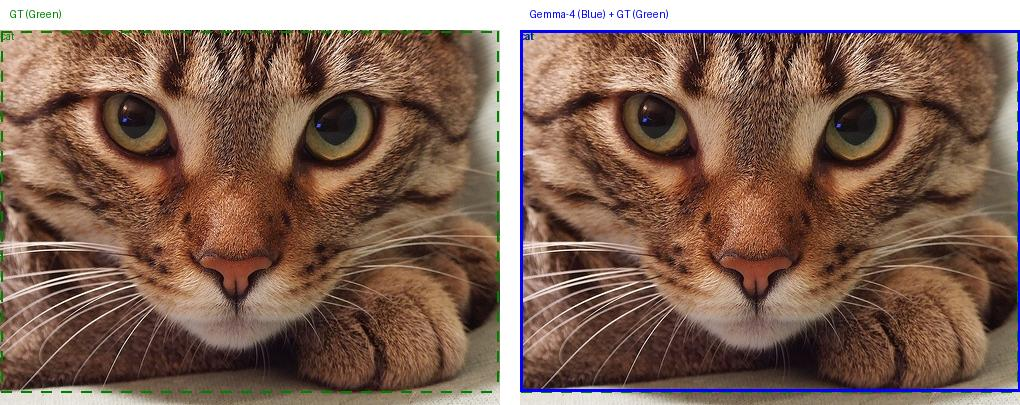
\includegraphics[width=0.95\textwidth]{figures/compare_000542.jpg}
    \caption{成功案例：cat 检测。Gemma-4 的蓝色框与 GT 绿色虚线几乎完全重合，对应 cat 类 90.89\% AP。大物体 + 语义特征鲜明是 VLM 零样本检测的最优场景。}
    \label{fig:compare_cat}
\end{figure}

\begin{figure}[H]
    \centering
    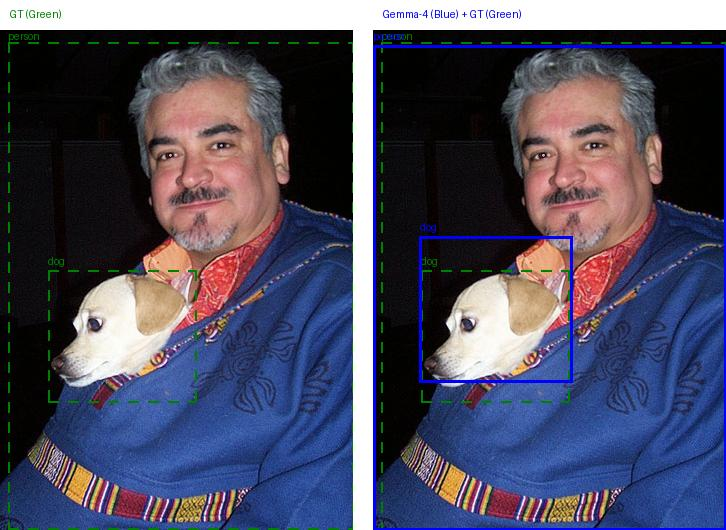
\includegraphics[width=0.95\textwidth]{figures/compare_000001.jpg}
    \caption{定位偏差案例：person + dog。Gemma-4 正确识别了两个类别，但 person 框包含了整张图（远大于 GT），dog 框也偏大。反映了 2.3B 小模型空间定位精度不足的问题。}
    \label{fig:compare_person_dog}
\end{figure}

\begin{figure}[H]
    \centering
    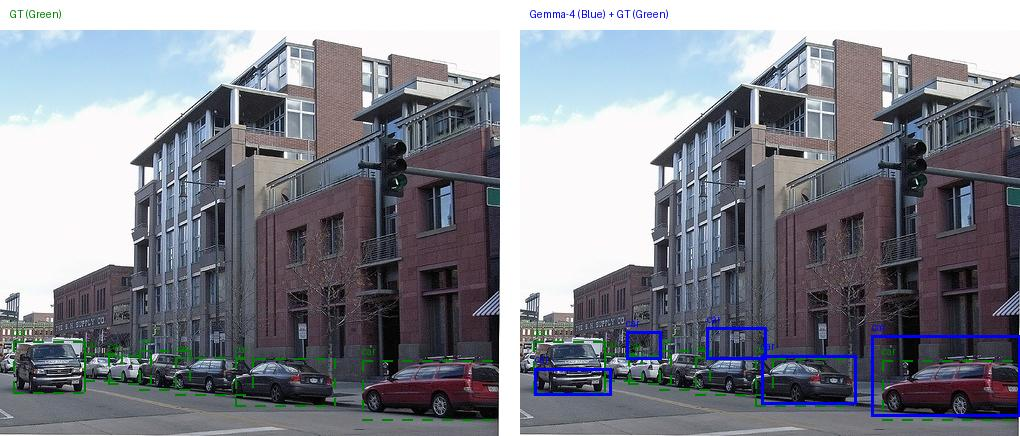
\includegraphics[width=0.95\textwidth]{figures/compare_000004.jpg}
    \caption{密集场景漏检案例：多车 + 行人。GT 标注 7 个目标（多辆 car + person），Gemma-4 仅检测到 5 个，遗漏了较小的目标。这是 VLM 自回归生成在密集实例场景下的典型短板。}
    \label{fig:compare_dense}
\end{figure}

\subsection{对比分析}

\textbf{Gemma-4 接近或超越 PLN 的类别}：cat (+0.90), dog ($-$0.85)。cat 是唯一 Gemma-4 超过 PLN 的类别（90.89\% vs 89.99\%），dog 几乎持平。这两个类别在互联网图像中的出现频率极高，VLM 在预训练阶段积累了大量相关视觉-语义知识。值得注意的是，PLN 的 cat AP（89.99\%）已经非常高，Gemma-4 能在完全零样本的条件下超过这个数字，说明 VLM 对语义特征鲜明的大物体具备超越专用检测器的识别能力。

\textbf{PLN 大幅领先的类别（差距 $>$ 20 点）}：diningtable ($-$34.89), sofa ($-$30.25), tvmonitor ($-$26.95), car ($-$24.43), boat ($-$23.81), bicycle ($-$20.53), aeroplane ($-$19.99)。失败原因可归纳为三类：

\begin{enumerate}
    \item \textbf{边界模糊的家居物品}（diningtable, sofa）：这类物体的边界在视觉上不清晰，VLM 难以确定精确的 bounding box 范围，框往往过大或过小。PLN 通过有监督训练直接学习了这些类别的边界模式。
    \item \textbf{密集/远景目标}（boat, car）：图像中出现多个同类小目标时，VLM 倾向于只检测最显著的几个，导致大量漏检。这是自回归生成范式的固有限制——每多输出一个框就多消耗数十个 token。
    \item \textbf{需要精确边界的物品}（tvmonitor, bicycle）：这些物体的检测质量高度依赖框的精确性，VLM 的坐标回归精度不如经过有监督训练的关键点回归。
\end{enumerate}

\subsection{范式差异的本质}

两种方法在能力维度上呈现清晰的互补特征：

\begin{table}[H]
\centering
\caption{两种检测范式的能力维度对比}
\label{tab:capability}
\begin{tabular}{@{}lcc@{}}
\toprule
\textbf{能力维度} & \textbf{PLN (有监督)} & \textbf{Gemma-4 (零样本)} \\
\midrule
空间定位精度 & 强（直接学习坐标回归） & 弱（离散化文本输出） \\
语义理解 & 受限于训练集分布 & 强（海量预训练知识） \\
密集实例检测 & 中（受限于网格容量） & 弱（自回归生成瓶颈） \\
开放词汇能力 & 无（固定 20 类） & 有（任意自然语言类别） \\
推理效率 & 高（$\sim$30 ms） & 低（$\sim$4370 ms） \\
标注成本 & 高（需大量 bbox 标注） & 零 \\
\bottomrule
\end{tabular}
\end{table}

PLN 的核心优势在于\textbf{精确的空间定位能力}：通过关键点检测和链接回归，直接在特征图上学习坐标映射。这种能力是通过在 16k+ 张标注图像上迭代数万次获得的。

Gemma-4 的核心优势在于\textbf{强大的语义理解}：不需要看过任何 VOC 标注就"知道" cat 长什么样，并能给出 90.89\% 的 AP。这种能力来自大规模视觉-语言预训练中积累的通用视觉知识。

17.23 个 mAP 点的差距，本质上是"通用智能的零样本泛化"与"任务特化的精确拟合"之间的 trade-off。考虑到 PLN 使用了完整的有监督训练（16k+ 张标注图像、200 个 epoch、3.3 小时 GPU 训练），而 Gemma-4 完全是零样本（零标注、零训练、仅一句 prompt），这个差距说明 VLM 的视觉基础能力已经达到了相当可观的水平。

% ============================================================
\section{讨论}

\subsection{51.51\% 零样本 mAP 的位置}

将 Gemma-4 E2B 的 51.51\% 放在 VOC 2007 检测的历史脉络中：

\begin{itemize}
    \item 随机基线（均匀猜测 + 随机框）：约 1--2\% mAP
    \item DPM v5（2010, 传统特征）：33.7\% mAP
    \item R-CNN（2014, 深度学习开端）：58.5\% mAP
    \item \textbf{Gemma-4 E2B（2025, 零样本）}：\textbf{51.51\% mAP}
    \item PLN-ResNet18（2017 架构, 有监督）：68.74\% mAP
    \item Faster R-CNN + ResNet-101（2016, 有监督）：76.4\% mAP
\end{itemize}

一个 2.3B 参数的通用模型，在没有看过任何 VOC 标注的情况下，达到了介于 DPM v5 和 R-CNN 之间的性能。考虑到 DPM v5 是专门为目标检测设计的方法，而 R-CNN 开创了深度学习检测的新纪元，Gemma-4 E2B 的零样本表现处于一个有意义的位置。

\subsection{瓶颈分析}

\textbf{空间定位精度}：VLM 生成的坐标是离散化到 1000$\times$1000 网格的整数，理论最大精度约 0.1\%。但实际瓶颈不在此——2.3B 模型的视觉编码器分辨率有限，对小目标的定位误差远大于网格精度。IoU 阈值敏感性分析（表~\ref{tab:iou_sensitivity}）直接验证了这一点：mAP 从 0.5 到 0.75 阈值下降 41.7\%，远高于有监督检测器的典型降幅（15--25\%）。错误分析进一步表明，12.4\% 的检测框属于"定位误差"类型（正确类别但 IoU 不足），如果框的精度能提升到 IoU$\geq$0.5，mAP 将显著改善。

\textbf{密集实例检测}：当一张图中同类物体超过 3--4 个时（如一群人、一排瓶子），模型倾向于只输出最显著的几个。错误分析（表~\ref{tab:gt_recall}）显示 29.7\% 的 GT 框未被检测到，其中 person 类漏检 1,278 个（占 person GT 的 28.2\%），是漏检最严重的类别。这是 VLM 自回归生成范式的固有限制——每多输出一个框就多消耗数十个 token，而模型在生成过程中会倾向于"及时停止"。

\textbf{推理效率}：4.37s/张的速度使其无法用于任何实时场景。这是 VLM 做检测的根本 trade-off：获得了零样本泛化能力，但牺牲了两个数量级的推理效率。在自动驾驶等对延迟敏感的场景中，这一差距目前是不可接受的。

\subsection{潜在改进方向}

以下方向可能提升零样本 mAP，但本次评测严格遵循零样本约束，未做实验：

\begin{enumerate}
    \item \textbf{更大模型}：Gemma 4 E4B 或 26B-A4B 预期能提升 5--15 个 mAP 点，但推理成本也会相应增加。
    \item \textbf{CoT prompt}：引导模型先描述图像内容再输出检测框，可能提升小目标召回率，但推理时间会翻倍。
    \item \textbf{多轮检测}：先检测大物体，再通过追问"还有其他小物体吗？"补充遗漏，可能改善密集实例的召回。
    \item \textbf{框级置信度}：当前使用序列级 log-prob 作为所有框的统一置信度，若能实现框级打分，如通过额外 prompt 让模型为每个框打分，可能改善 PR 曲线排序质量。
\end{enumerate}

% ============================================================
\section{结论}

本报告完成了两项工作：Gemma-4 E2B（2.3B 有效参数）在 Pascal VOC 2007 test 集上的零样本目标检测评测，以及与第一阶段 PLN-ResNet18 的跨范式对比分析。主要结论如下：

\begin{enumerate}
    \item \textbf{零样本检测达到可用水平}：mAP@0.5 = 51.51\%，mAP@0.75 = 30.05\%，4952 张图推理成功率 99.5\%，仅 1 张解析失败。
    \item \textbf{语义理解可超越专用检测器}：对语义特征鲜明的大物体（cat 90.89\%, dog 82.70\%），Gemma-4 接近甚至超过有监督训练的 PLN。
    \item \textbf{空间定位是核心短板}：mAP 从 @0.5 到 @0.75 下降 41.7\%，远高于有监督检测器的典型降幅。错误分析显示 29.7\% 的 GT 被漏检，16.8\% 的检测框为背景误检（幻觉），定位误差占 12.4\%。
    \item \textbf{两种范式互补而非替代}：有监督检测器擅长精确定位和高效推理，VLM 擅长语义理解和零样本泛化。17.23 个 mAP 点的差距在快速缩小。
    \item \textbf{推理效率差距约 145 倍}：自回归生成 vs 前向传播，这是范式差异的必然代价，短期内难以弥合。
\end{enumerate}

从更宏观的视角看，这两个阶段的任务共同描绘了目标检测领域的范式演进图景：从精心设计的专用架构（PLN 的关键点检测 + 链接回归）到通用视觉语言模型的零样本能力（Gemma-4 的 prompt 驱动检测）。前者代表了"为每个任务训练一个专用模型"的传统范式，后者代表了"一个通用模型解决所有视觉任务"的新范式。当前两种范式各有优势，但趋势清晰：随着 VLM 规模增大和推理优化，通用模型的精度天花板在不断抬升，而其零标注、零训练的核心优势是专用检测器无法匹敌的。

% ============================================================
\appendix
\section{实验环境}

\begin{table}[H]
\centering
\begin{tabular}{@{}ll@{}}
\toprule
\textbf{项} & \textbf{配置} \\
\midrule
GPU & NVIDIA RTX 4090 (24GB VRAM) \\
精度 & BF16 \\
Python & 3.10 \\
PyTorch & 2.1 \\
CUDA & 12.1 \\
Transformers & latest \\
模型 & google/gemma-4-E2B-it (Apache 2.0) \\
解码策略 & Greedy (do\_sample=False) \\
max\_new\_tokens & 2048 \\
\bottomrule
\end{tabular}
\end{table}


% ============================================================
\begin{thebibliography}{9}

\bibitem{gemma4}
Gemma Team, Google. \textit{Gemma 4 Technical Report}. 2025.

\bibitem{voc}
Everingham, M., Van Gool, L., Williams, C. K., Winn, J., \& Zisserman, A. The Pascal Visual Object Classes (VOC) Challenge. \textit{IJCV}, 88(2), 303--338, 2010.

\bibitem{pln}
Wang, X., Chen, K., Huang, Z., Yao, C., \& Liu, W. Point Linking Network for Object Detection. \textit{arXiv preprint arXiv:1706.03646}, 2017.

\bibitem{rcnn}
Girshick, R., Donahue, J., Darrell, T., \& Malik, J. Rich Feature Hierarchies for Accurate Object Detection and Semantic Segmentation. \textit{CVPR}, 2014.

\bibitem{fasterrcnn}
Ren, S., He, K., Girshick, R., \& Sun, J. Faster R-CNN: Towards Real-Time Object Detection with Region Proposal Networks. \textit{NeurIPS}, 2015.

\bibitem{resnet}
He, K., Zhang, X., Ren, S., \& Sun, J. Deep Residual Learning for Image Recognition. \textit{CVPR}, 2016.

\end{thebibliography}

\end{document}
